\begin{frame}
  \frametitle{Hybrid $S_N$-Diffusion Method: Preliminary Results}
  \textbf{Illustration of the Hybrid Method With Case 0} \\
  \begin{columns}
    \column[t]{5.5cm}
    \textbf{Problem Description}
    \begin{itemize}
      \item 1-D, two-region system consisting of:
      \begin{itemize}
        \item 0.5-cm thick control rod region
        \item 19.5-cm thick homogenized mixture of molten fuel salt and graphite moderator
      \end{itemize}
      \item Material compositions of the Molten Salt Reactor Experiment (MSRE)
      \item Two-group constants are sampled at 900 K and generated using OpenMC
    \end{itemize}
    \column[t]{5.5cm}
    \begin{figure}[htb!]
      \centering
      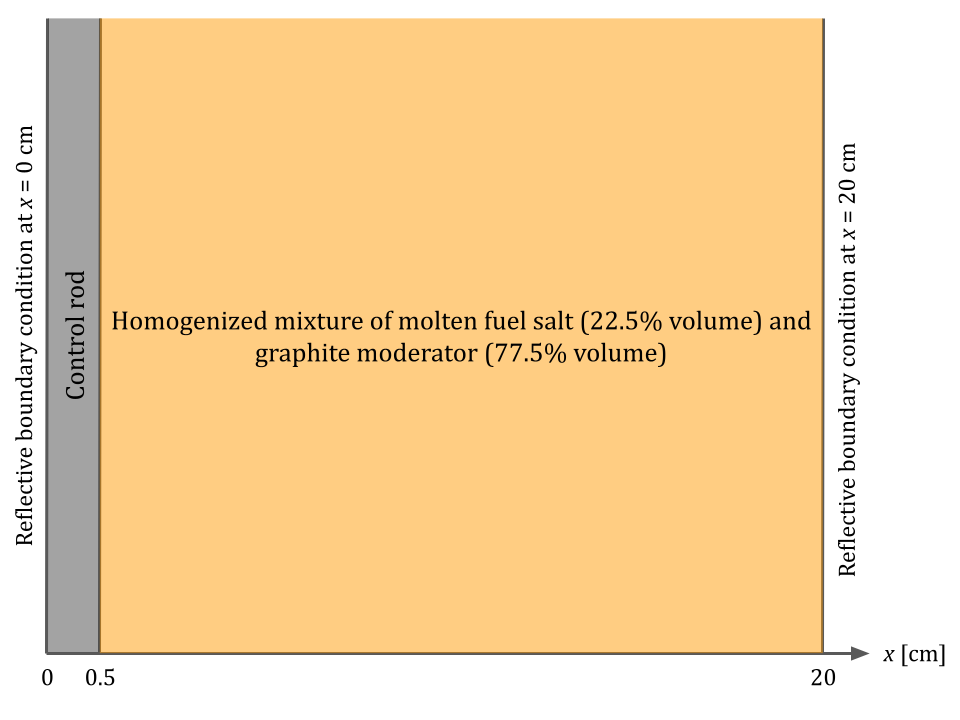
\includegraphics[width=\columnwidth]{../images/case-0-geometry}
      \caption{Case 0 problem geometry.}
      \label{fig:case-0-geom}
    \end{figure}
  \end{columns}
\end{frame}

\begin{frame}
  \frametitle{Hybrid $S_N$-Diffusion Method: Preliminary Results}
  \textbf{Illustration of the Hybrid Method With Case 0}
  \vspace{.3cm}

  I solved for the neutron flux in Case 0 using the following set of numerical solvers:
  \begin{enumerate}
    \item Neutron diffusion solver with $P_1$-based diffusion coefficients generated directly from
      the group constants generation step with OpenMC
    \item $S_N$ neutron transport solver with $N=8$ and up to 2nd-order anisotropic scattering
      cross sections
    \item Neutron diffusion solver with SVDCs generated from the prior $S_8$ flux solution
    \item Hybrid $S_N$-Diffusion solver with $\Omega^d_1$ spanning from $x=0$ cm to $x=17.5$ cm
  \end{enumerate}

  The neutron diffusion and $S_N$ solvers are implemented in Python using the finite difference
  method and diamond difference method, respectively.
\end{frame}

\begin{frame}
  \frametitle{Hybrid $S_N$-Diffusion Method: Preliminary Results}
  \textbf{Case 0 Results}
  \begin{figure}
    \centering
    \begin{subfigure}[b]{.49\textwidth}
      \centering
      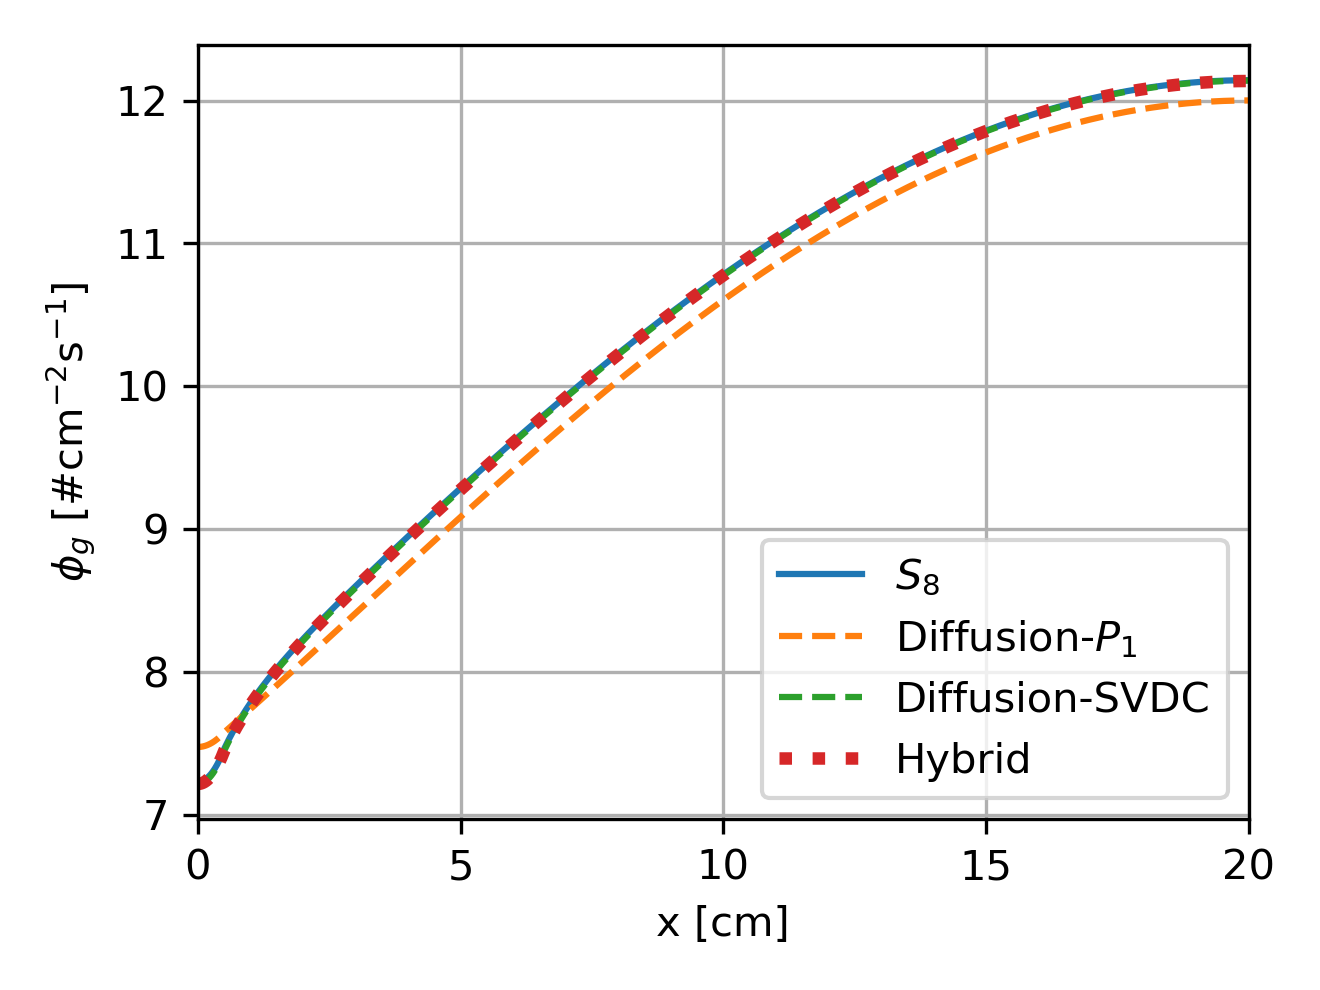
\includegraphics[width=\textwidth]{../images/case-0-group-1-hybrid-flux}
      \caption{Group 1}
      \label{fig:c0g1hf}
    \end{subfigure}
    \hfill
    \begin{subfigure}[b]{.49\textwidth}
      \centering
      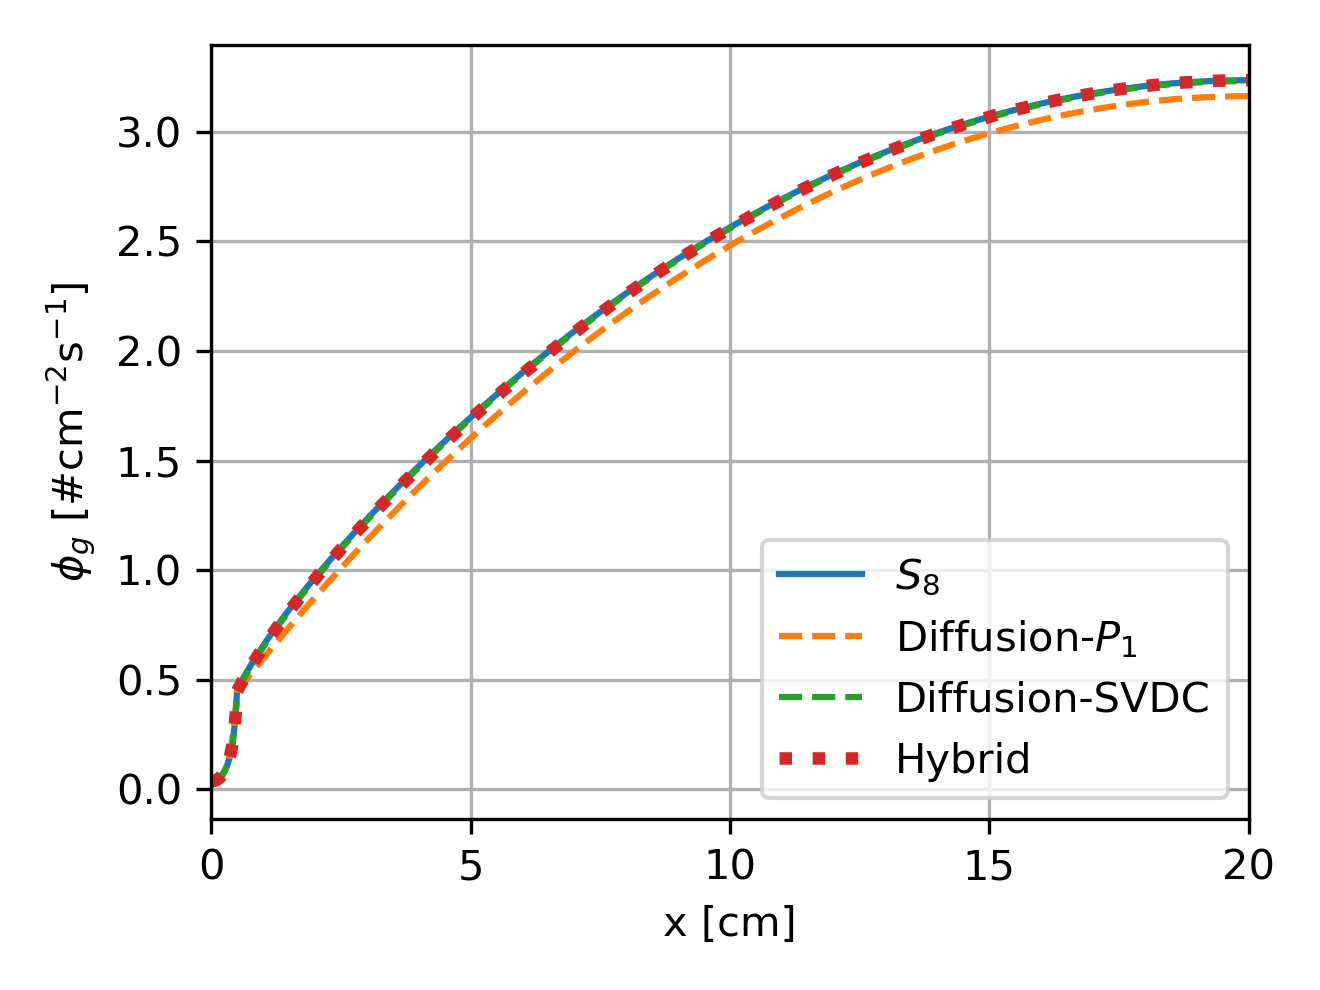
\includegraphics[width=\textwidth]{../images/case-0-group-2-hybrid-flux}
      \caption{Group 2}
      \label{fig:c0g2hf}
    \end{subfigure}
    \caption{Neutron group 1 and 2 flux distributions from the diffusion, $S_8$, reference
    \gls{SVDC}, and hybrid methods for Case 0.}
  \end{figure}
\end{frame}

\begin{frame}
  \frametitle{Hybrid $S_N$-Diffusion Method: Preliminary Results}
  \textbf{Case 0 Results}
  \begin{figure}
    \centering
    \begin{subfigure}[b]{.49\textwidth}
      \centering
      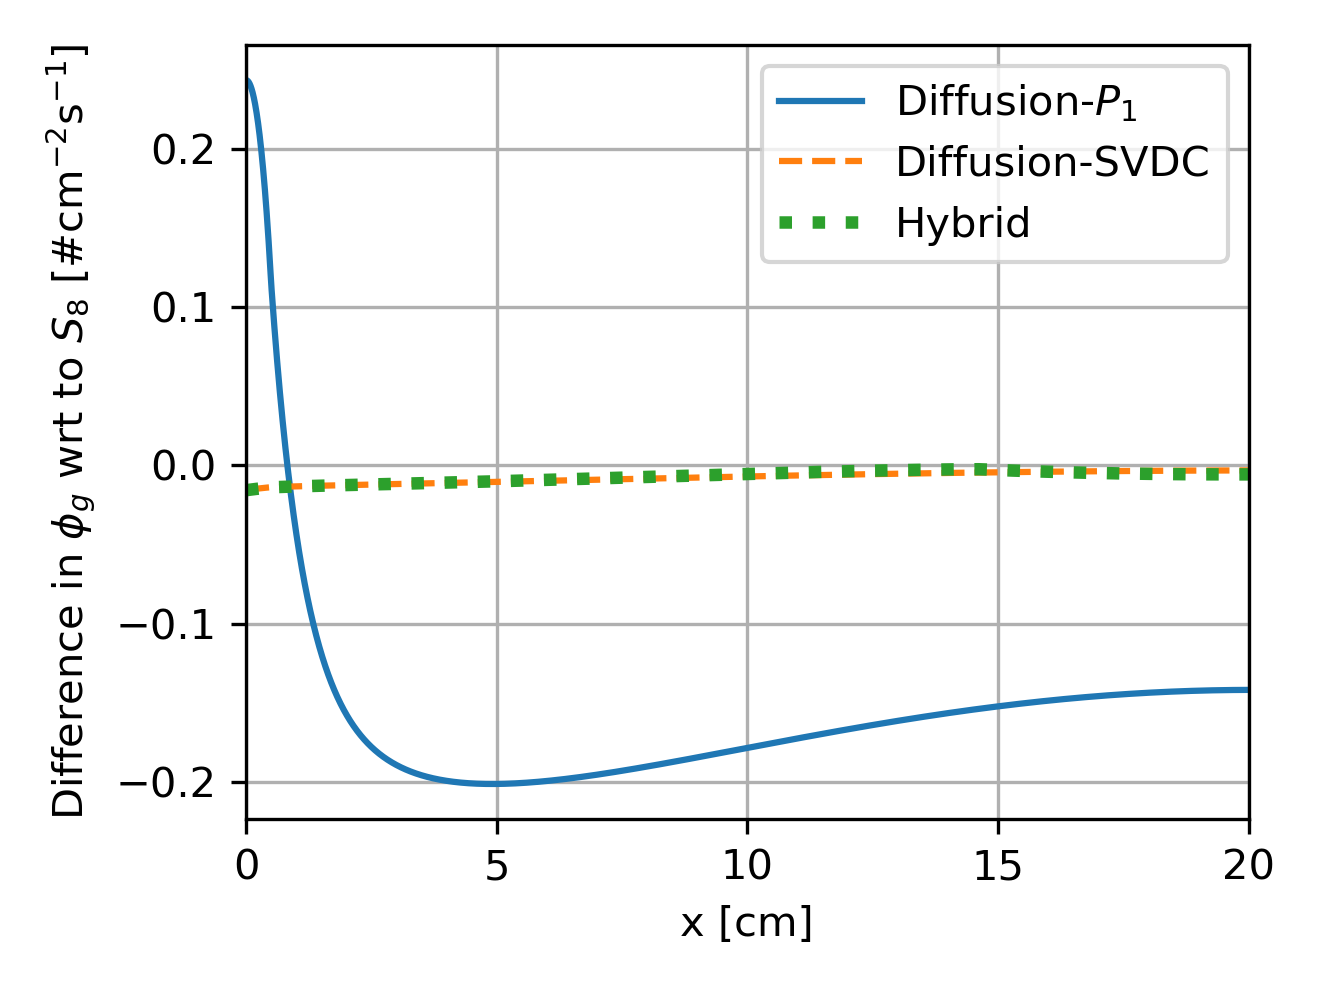
\includegraphics[width=\textwidth]{../images/case-0-group-1-hybrid-flux-diff}
      \caption{Group 1}
      \label{fig:c0g1hfdiff}
    \end{subfigure}
    \hfill
    \begin{subfigure}[b]{.49\textwidth}
      \centering
      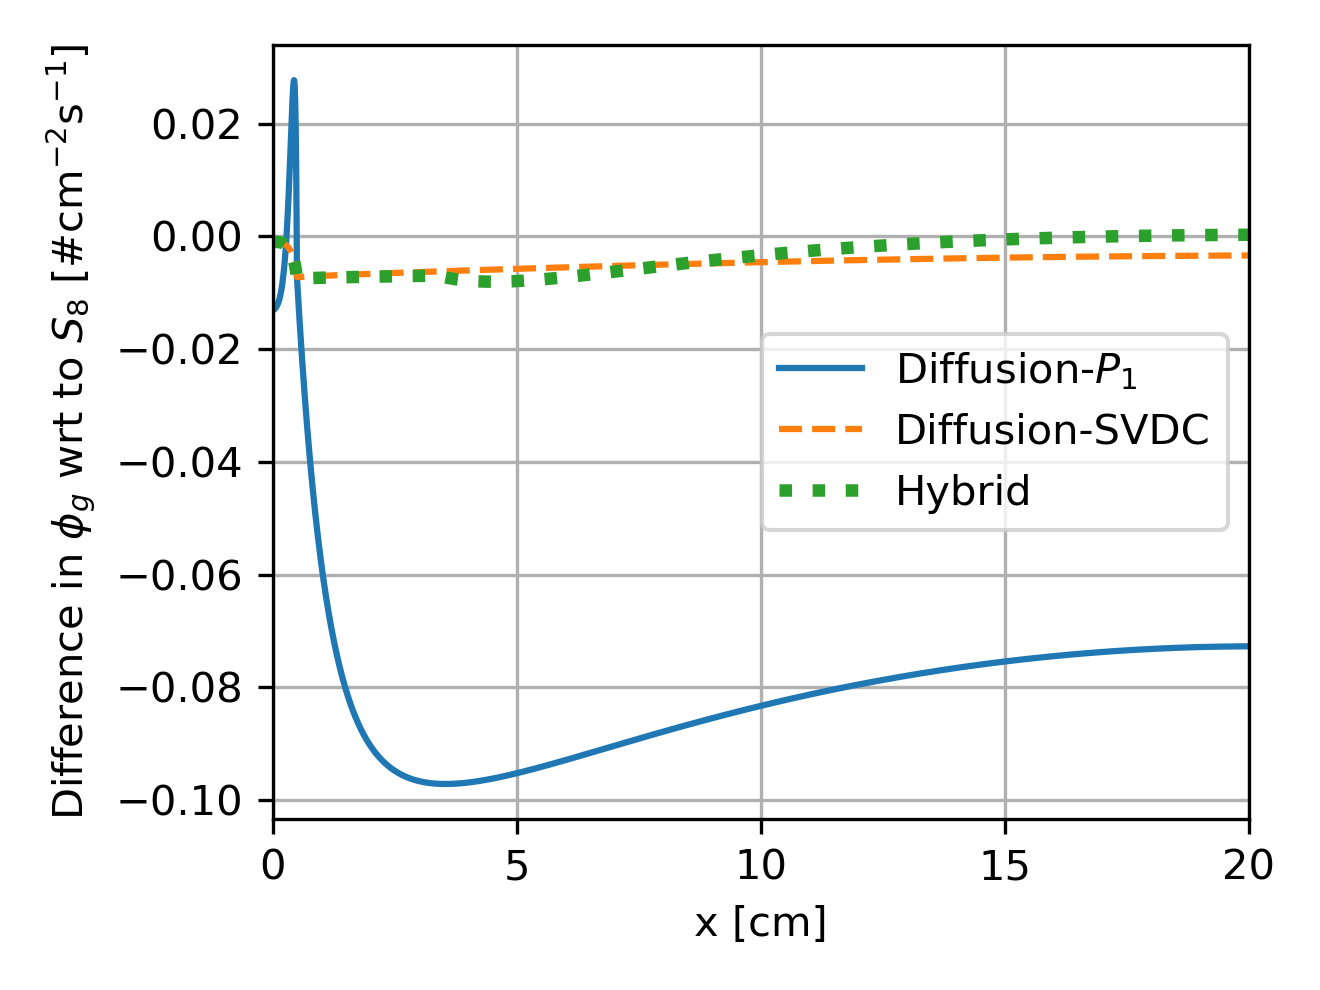
\includegraphics[width=\textwidth]{../images/case-0-group-2-hybrid-flux-diff}
      \caption{Group 2}
      \label{fig:c0g2hfdiff}
    \end{subfigure}
    \caption{Difference in neutron group 1 and 2 flux distributions from the diffusion,
    diffusion-\gls{SVDC}, and hybrid methods with respect to the $S_8$ flux distribution for Case 0.}
    \label{fig:c0hfdiff}
  \end{figure}
\end{frame}

\begin{frame}
  \frametitle{Hybrid $S_N$-Diffusion Method: Preliminary Results}
  \textbf{Case 0 Results}
  \begin{table}
    \centering
    \caption{Multiplication factor $k$ estimates from the diffusion-$P_1$, $S_8$, and
    diffusion-\gls{SVDC} solvers and the absolute difference relative to the $S_8$ estimate.}
    \begin{tabular}{l S S}
      \toprule
      Solver type & {$k$} & {$k-k_{S8}$} \\
      \midrule
      $S_8$ & 0.62736 & {-} \\
      Diffusion-$P_1$ & 0.60890 & -0.01846 \\
      Diffusion-\gls{SVDC} & 0.62750 & +0.00013 \\
      Hybrid & 0.62774 & +0.00038 \\
      \bottomrule
    \end{tabular}
    \label{table:c0k}
  \end{table}
\end{frame}

\begin{frame}
  \frametitle{Hybrid $S_N$-Diffusion Method: Preliminary Results}
  \textbf{Case 0 Results}
  \begin{figure}[htb!]
    \centering
    \begin{subfigure}[b]{.49\textwidth}
      \centering
      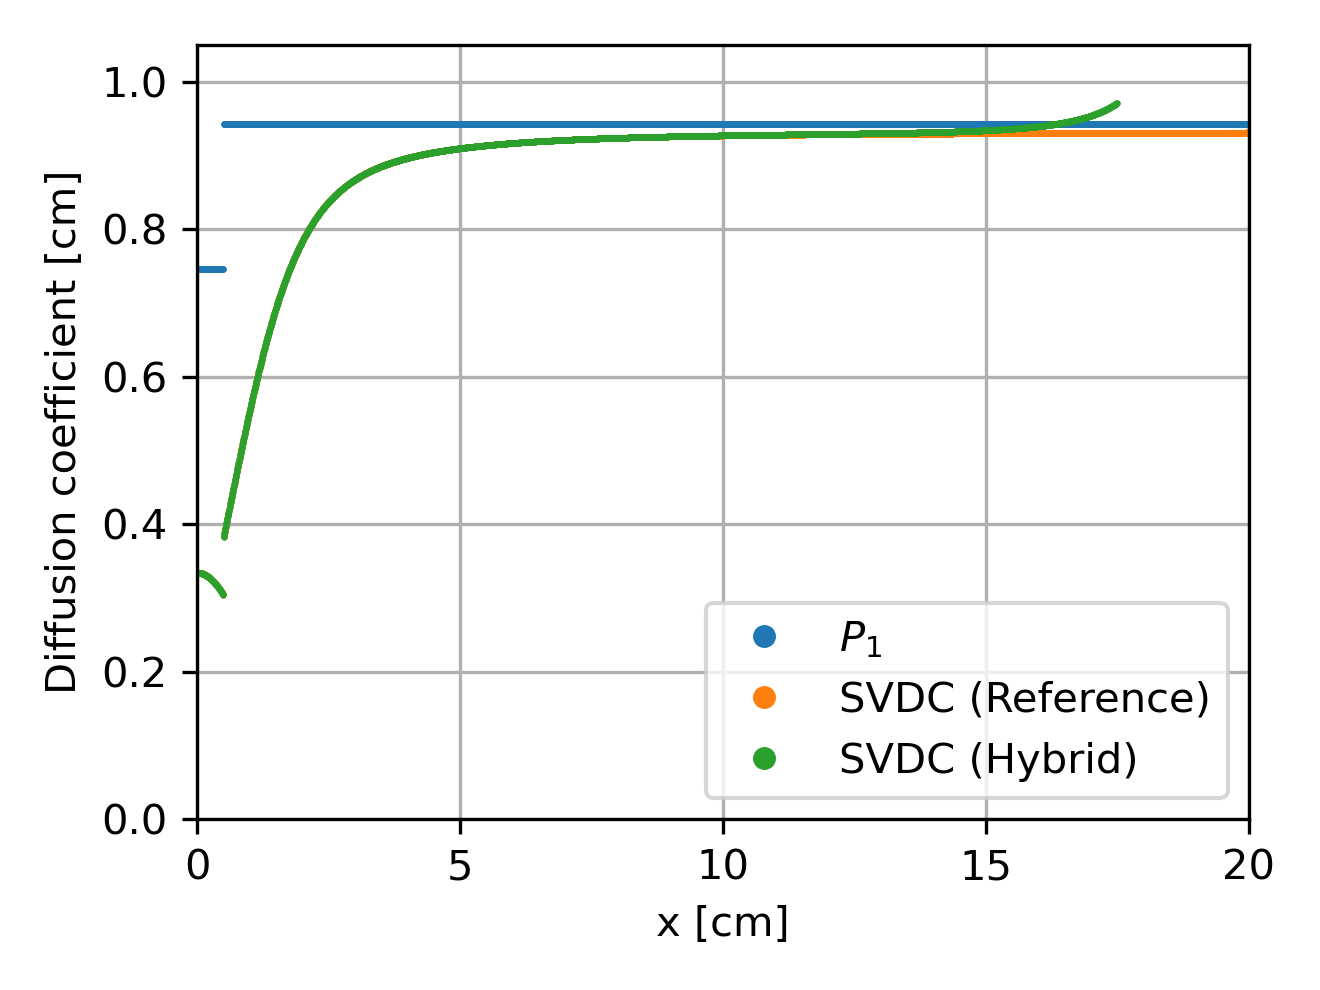
\includegraphics[width=\textwidth]{../images/case-0-group-1-hybrid-diffcoef}
      \caption{Group 1}
      \label{fig:c0g1hd}
    \end{subfigure}
    \hfill
    \begin{subfigure}[b]{.49\textwidth}
      \centering
      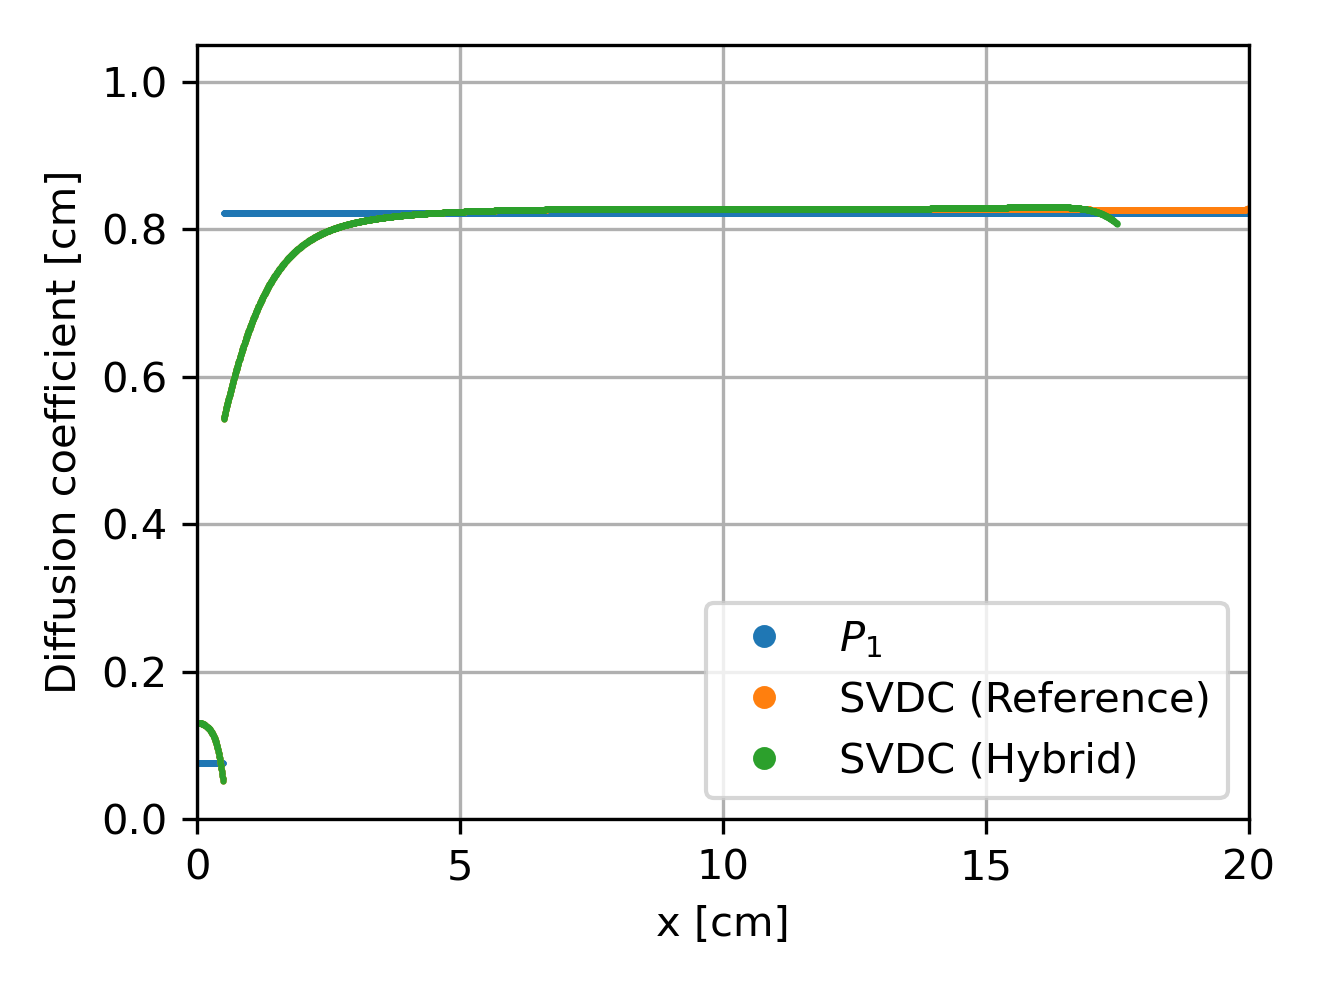
\includegraphics[width=\textwidth]{../images/case-0-group-2-hybrid-diffcoef}
      \caption{Group 2}
      \label{fig:c0g2hd}
    \end{subfigure}
    \caption{$P_1$-based flux-limited diffusion coefficient and \gls{SVDC} spatial distribution for
    Case 0. The \gls{SVDC} distributions were generated from the reference $S_8$ (``SVDC'') and the
    hybrid (``Hybrid'') calculations.}
    \label{fig:c0hd}
  \end{figure}
\end{frame}

\begin{frame}
  \frametitle{Hybrid $S_N$-Diffusion Method: Preliminary Results}
  \textbf{Case 0 Discussion}
  \begin{itemize}
    \item The hybrid method automatically determines the buffer zone size by comparing the SVDCs
      to the $P_1$ diffusion coefficient values.
    \item The hybrid method converges rapidly within two outer iterations.
    \item The required size of $\Omega^d_1$ for Case 0 is large because the control rod region is
      the only significant source of influence on the neutron flux.
    \item $\Omega^d_1$ is smaller for more realistic reactor systems which are more heterogeneous
      and have vacuum boundary conditions.
  \end{itemize}
\end{frame}

\begin{frame}
  \frametitle{Hybrid $S_N$-Diffusion Method: Preliminary Results}
  \textbf{Further 1-D Test Cases}
  \begin{figure}[htb!]
    \centering
    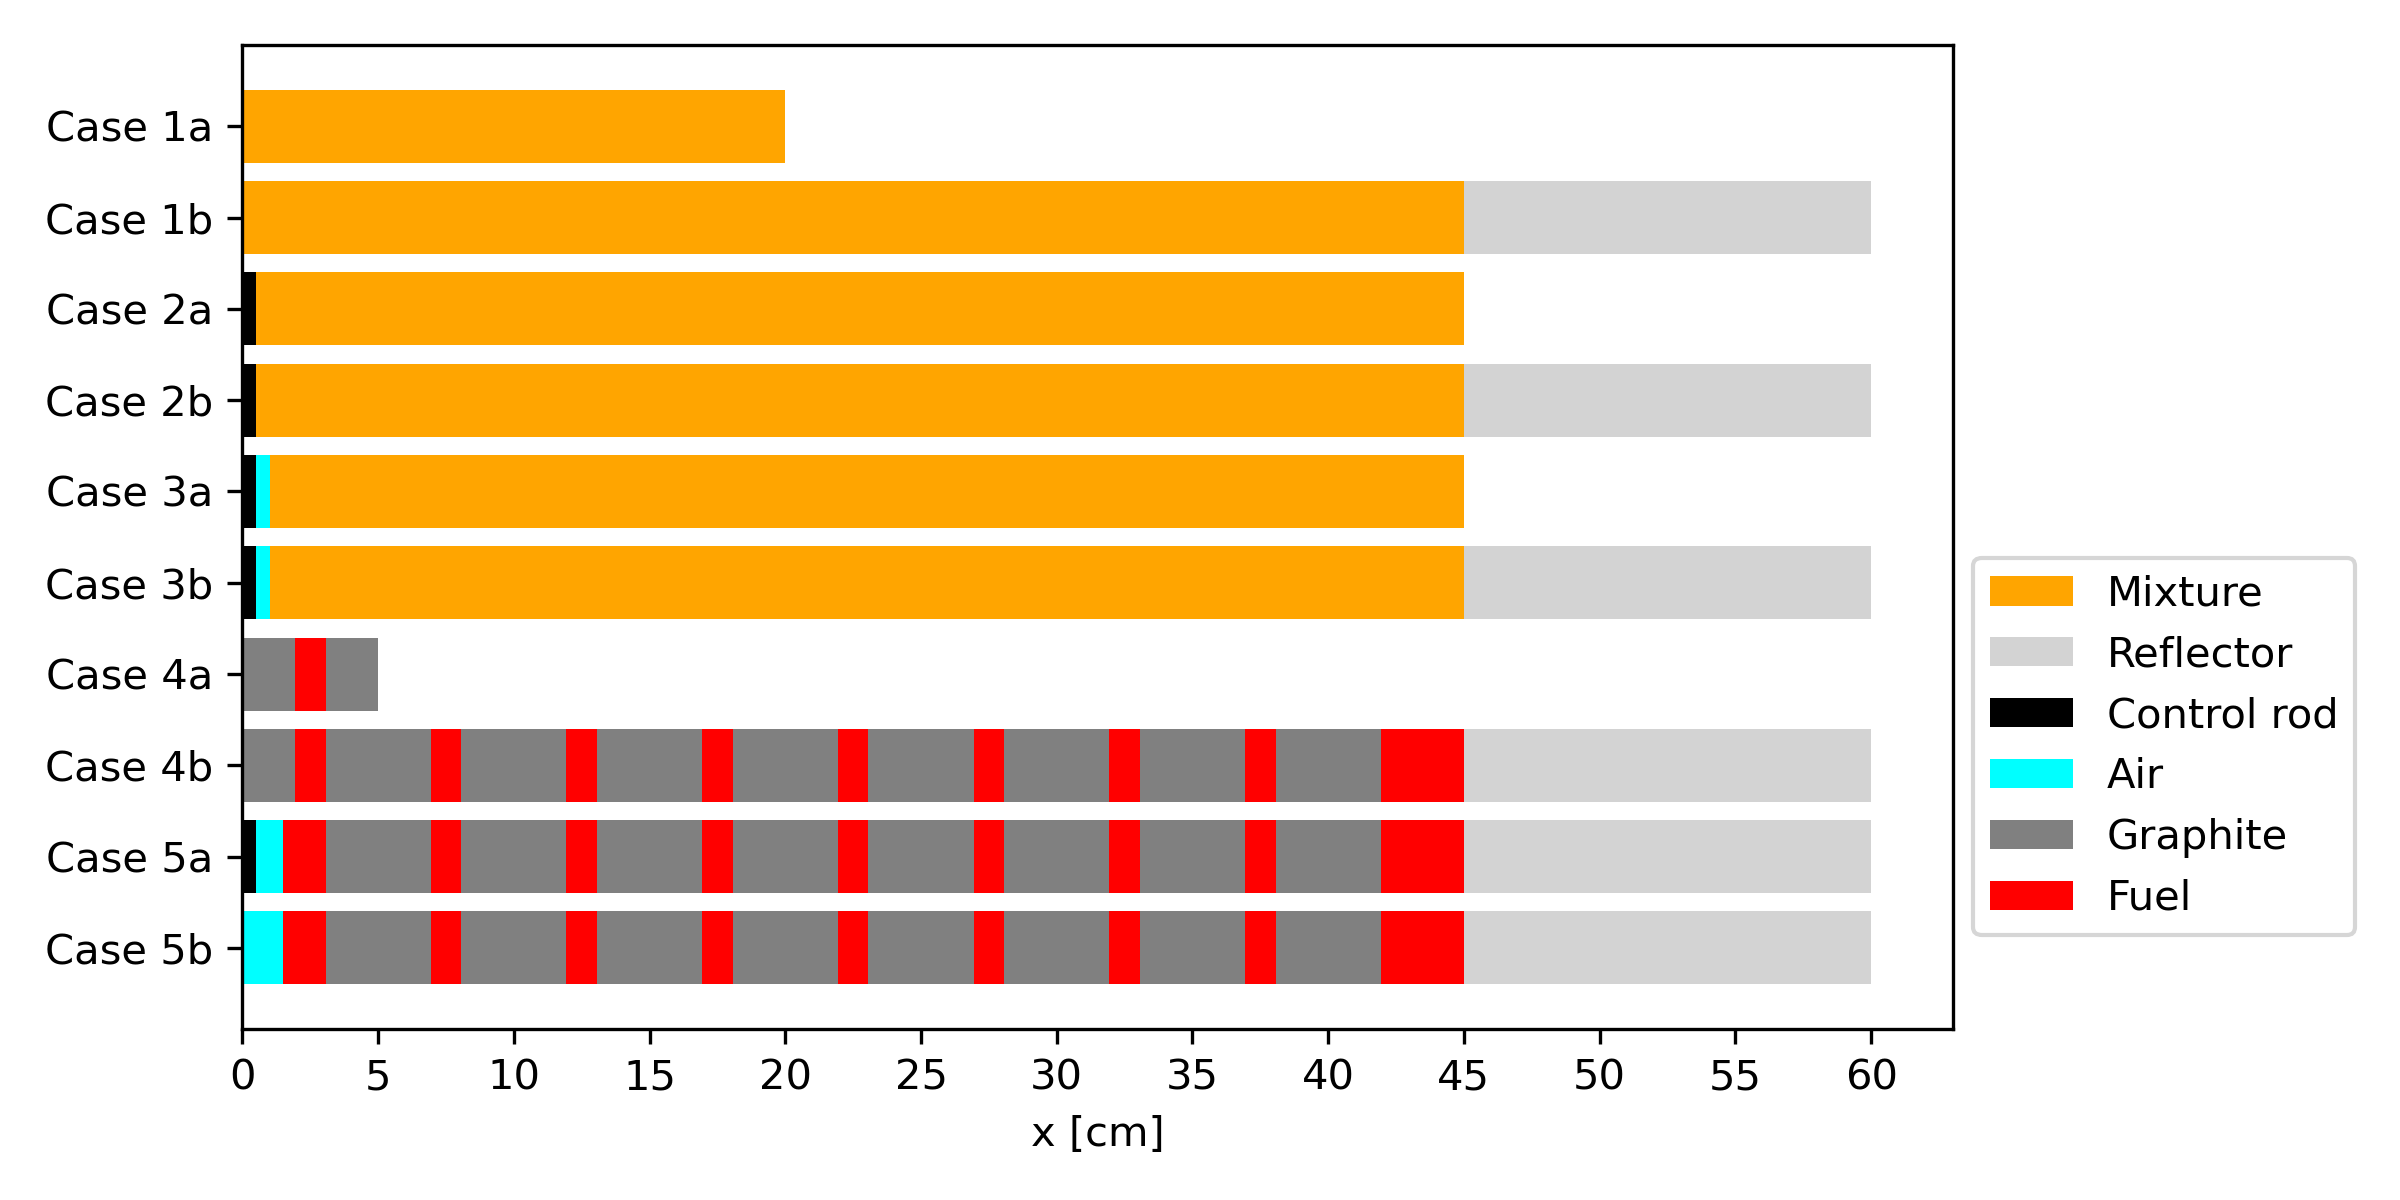
\includegraphics[width=\columnwidth]{case-geometry}
    \caption{Geometries of the 1-D test cases. The material labeled ``mixture'' represents a
      homogeneous mixture of fuel and graphite at a ratio of 22.5\%-77.5\% by volume. All geometries
      have reflective boundary conditions on the boundary at $x=0$ cm. The right-side boundaries are
      reflective for Cases 1a, 2a, 3a, and 4a, and vacuum for Cases 1b, 2b, 3b, 4b, 5a, and 5b.}
    \label{fig:case-geom}
  \end{figure}
\end{frame}
